\documentclass[
  11pt,
  letterpaper,
   addpoints,
  answers
  ]{exam}

% Carga el preámbulo localizado en la carpeta superior
\NeedsTeXFormat{LaTeX2e}[2023/04/30]

% Provide the name of your page, the date it was last updated, and a comment about what it's used for
\ProvidesPackage{../exercise-preamble}[2023/04/30 Prof. Cassanelli custom LaTeX style]

% \usepackage{printlen}
% \uselengthunit{in}\printlength{\textwidth}

% PACKAGES
\usepackage[dvipsnames]{xcolor}

\usepackage{graphicx}
\graphicspath{{../figures}}
\usepackage{amsmath,amsthm,amssymb,mathtools,mathrsfs}
\usepackage{commath}
\usepackage{upgreek}
\usepackage{cancel}
\usepackage{enumerate}
\usepackage[font=small]{caption}
\usepackage[normalem]{ulem}
\usepackage{steinmetz}

\usepackage[left=1.5cm, right=1.5cm, top=1cm]{geometry}

% REFERENCES AND OTHERS
\usepackage{../aas_macros}
\usepackage{natbib}
\bibpunct{(}{)}{;}{a}{}{,}

\usepackage{tikz}
\usepackage{tikz-3dplot}
\usepackage{circuitikz}
\usepackage{pgfplots}
\pgfplotsset{compat=1.15}
\usepgfplotslibrary{smithchart}
\usetikzlibrary{
  decorations.pathmorphing,
  decorations.markings,
  calc,
  patterns,
  decorations,
  angles,
  quotes,
  ext.topaths.arcthrough,
  shapes
  }

\usepackage{siunitx}
\sisetup{
    range-phrase=\text{--},
    range-units=single,
    separate-uncertainty=true,
    print-unity-mantissa=false
    }
\DeclareSIUnit{\gauss}{G}
\DeclareSIUnit{\jansky}{Jy}

\newcommand{\iu}{\mathrm{i}\mkern1mu}
\newcommand{\ju}{\mathrm{j}\mkern1mu}
\newcommand{\euler}{\mathrm{e}}
\newcommand{\exponential}[1]{\mathrm{exp}\left[#1\right]}
\newcommand{\uvec}[1]{\widehat{\mathbf{#1}}}
\newcommand{\uvecs}[1]{\boldsymbol{\widehat{#1}}}
\newcommand{\bvec}[1]{\boldsymbol{\mathcal{#1}}}

\usepackage{hyperref}
\hypersetup{
    % bookmarks=true,
    unicode=true,
    pdftoolbar=true,
    pdfmenubar=true,
    pdffitwindow=false,
    pdfstartview={FitH},
    pdftitle={EL3103},
    pdfauthor={Tomas Cassanelli},
    pdfcreator={Tomas Cassanelli},
    pdfnewwindow=true,
    colorlinks=true,
    linkcolor=Violet,
    citecolor=Violet,
    urlcolor=Violet
    }

% Exam document class
\renewcommand{\figurename}{Figura}
\renewcommand{\tablename}{Cuadro}
\pagestyle{empty}

\usepackage[spanish]{cleveref}

\crefname{question}{\protect{pregunta}}{\protect{preguntas}}
\Crefname{question}{\protect{Pregunta}}{\protect{Preguntas}}
\creflabelformat{question}{#2{#1}#3}

\renewcommand{\solutiontitle}{\noindent\textbf{Solución:}\par\noindent}
\bracketedpoints
\pointname{~puntos}

\endinput

% Paquetes locales
\usepackage{float}
\usepackage{booktabs} % para \toprule, \midrule, \bottomrule
\usepackage{xcolor} % para colores
\usepackage{bm} % para negrita en símbolos matemáticos

% Macros locales
\newcommand{\Rel}{\mathfrak{R}} % símbolo para la reluctancia

\begin{document}

% Configuración del encabezado usando comandos de la clase exam
\pagestyle{headandfoot}
\extraheadheight{0.5in} % Baja el encabezado aumentando el espacio superior
\firstpageheader{\textit{Análisis de Sistemas Dinámicos y Estimación}}{}{EL3204-1}
\runningheader{\textit{Análisis de Sistemas Dinámicos y Estimación}}{}{EL3204}
\firstpagefooter{}{\thepage}{}
\runningfooter{}{\thepage}{}
\headrule % Línea debajo del encabezado

% Numeración de página
\pagenumbering{arabic}

% Portada
\begin{center}
    \vspace*{1cm}
    
    % Logo superior
    \includegraphics[width=0.5\textwidth]{../fcfm_die}
    
    \vspace{2cm}
    
    % Líneas decorativas superiores
    
\begin{tikzpicture}
        \draw[line width=2pt, black!70] (0,0) -- (10,0);
        \draw[line width=0.5pt, black!50] (0,0.2) -- (10,0.2);
    \end{tikzpicture}
    
    \vspace{1cm}
    
    % Título principal
    {\fontsize{28}{34}\selectfont\bfseries 
    Análisis de Sistemas\\[0.3cm]
    Dinámicos y Estimación}
    
    \vspace{0.5cm}
    
    {\Large\textbf{EL3204-1}}
    
    \vspace{1cm}
    
    % Líneas decorativas inferiores
    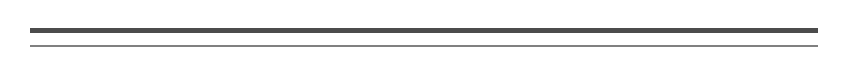
\begin{tikzpicture}
        \draw[line width=0.5pt, black!50] (0,0) -- (10,0);
        \draw[line width=2pt, black!70] (0,0.2) -- (10,0.2);
    \end{tikzpicture}
    
    \vspace{1.5cm}
    
    % Subtítulo
    {\LARGE\itshape Pauta Auxiliar 8 - Lema de Neyman-Pearson}
    
    \vspace{0.5cm}
    {\large Prof Marcos Orchard - Sebastian Espinoza.}\\
    {\large Prof Auxiliar Erik Sáez Aravena.}
    
    \vfill
    

    \vspace{1cm}
    
    % Decoración con ecuación diferencial de fondo
    \begin{tikzpicture}[remember picture, overlay]
        \node[opacity=0.08] at (current page.center) {
            \begin{tikzpicture}
                \node[font=\fontsize{120}{140}\selectfont, black!30] at (0,0) {$\dot{\mathbf{x}}$};
            \end{tikzpicture}
        };
    \end{tikzpicture}
    
    \vspace{1cm}
    
\end{center}

\newpage
%----------------------------
\section{Resumen}
El \textbf{Lema de Neyman-Pearson} es un resultado fundamental en teoría de detección que caracteriza el test óptimo para distinguir entre dos hipótesis simples. Dado un problema de detección binaria:
\begin{align*}
\mathcal{H}_0: & \quad X \sim f_{X_1^n}(x_1, ..., x_n|\theta = 0) \\
\mathcal{H}_1: & \quad X \sim f_{X_1^n}(x_1, ..., x_n|\theta = 1)
\end{align*}

donde $L(x_1^n|\theta)$ representa la \textbf{función de verosimilitud}:

\begin{itemize}
\item \textbf{Para variables continuas:}
\begin{equation}
L(x_1^n|\theta) = f_{X_1^n}(x_1, ..., x_n|\theta)
\end{equation}

\item \textbf{Para variables discretas:}
\begin{equation}
L(x_1^n|\theta) = P_{X_1^n}(X_1 = x_1, ..., X_n = x_n|\theta)
\end{equation}
\end{itemize}
Para un $\nu > 0$ arbitrario y una variable aleatoria binaria $\rho(w)$, se tiene que el test aleatorio de la forma:
\begin{equation}
\pi_\nu(w, x) = \begin{cases}
1 & \text{si } L(x|\theta = 1) > \nu L(x|\theta = 0) \\
0 & \text{si } L(x|\theta = 1) < \nu L(x|\theta = 0) \\
\rho(w) & \text{si } L(x|\theta = 1) = \nu L(x|\theta = 0)
\end{cases}
\end{equation}

es óptimo para su tamaño entre $[0, 1]$. Dado que $X$ es una variable aleatoria, el test se puede reescribir como una función de variable aleatoria notando que:
\begin{equation}
\pi_\nu(\rho, X) = \begin{cases}
1 & \text{si } L(X|\theta = 1) > \nu L(X|\theta = 0) \\
0 & \text{si } L(X|\theta = 1) < \nu L(X|\theta = 0) \\
\rho & \text{si } L(X|\theta = 1) = \nu L(X|\theta = 0)
\end{cases}
\end{equation}

con $\rho$ independiente de $X$. Además, el test de la forma (haciendo $\nu \to 0^+$):
\begin{equation}
(\forall x \in \mathbb{X})\pi(x) = 1
\end{equation}

es óptimo de tamaño 1 y el test de la forma (haciendo $\nu \to \infty$):
\begin{equation}
\pi(x) = \begin{cases}
1 & \text{si } L(x|\theta = 0) = 0 \\
0 & \text{si } L(x|\theta = 0) > 0
\end{cases}
\end{equation}
es óptimo de tamaño 0.

Para evaluar un test de detección $\pi: \mathbb{X} \mapsto \{0, 1\}$, usamos dos probabilidades fundamentales:

\textbf{Tamaño del test} (probabilidad de falsa alarma):
\begin{align}
\alpha_\pi &\triangleq P_{X_1^n}(\pi(X_1^n) = 1|\theta = 0) \nonumber \\
&= P_{X_1^n}(X_1^n \in \pi^{-1}(\{1\})|\theta = 0) \nonumber \\
&= \int_{\{(x_1,...,x_n)\in\mathbb{R}^n : \pi(x_1^n)=1\}} f_{X_1^n}(x_1,...,x_n|\theta = 0)dx_1...dx_n \nonumber \\
&= \mathbb{E}_{X_1^n}(\pi(X_1^n)|\theta = 0)
\end{align}

\textbf{Poder del test} (probabilidad de correcta detección de la hipótesis alternativa):
\begin{align}
\beta_\pi &\triangleq P_{X_1^n}(\pi(X_1^n) = 1|\theta = 1) \nonumber \\
&= P_{X_1^n}(X_1^n \in \pi^{-1}(\{1\})|\theta = 1) \nonumber \\
&= \int_{\{(x_1,...,x_n)\in\mathbb{R}^n : \pi(x_1^n)=1\}} f_{X_1^n}(x_1,...,x_n|\theta = 1)dx_1...dx_n \nonumber \\
&= \mathbb{E}_{X_1^n}(\pi(X_1^n)|\theta = 1)
\end{align}

Notar que $P_{X_1^n}(\pi(X_1^n) = 0|\theta = 1)$ es la probabilidad de no detección o el error de tipo II que corresponde precisamente a $1 - \beta_\pi$. El objetivo del Lema de Neyman-Pearson es \textbf{maximizar $\beta_\pi$ sujeto a que $\alpha_\pi \leq \alpha_0$}, donde $\alpha_0$ es un tamaño máximo permitido.


El cociente de verosimilitud mide qué tan ``favorable'' es la observación para $\mathcal{H}_1$ en comparación con $\mathcal{H}_0$:
\begin{itemize}
\item Si $L(x|\theta = 1) > \nu L(x|\theta = 0)$: la observación favorece fuertemente a $\mathcal{H}_1$ → decidimos $\mathcal{H}_1$ ($\pi = 1$)
\item Si $L(x|\theta = 1) < \nu L(x|\theta = 0)$: la observación favorece a $\mathcal{H}_0$ → decidimos $\mathcal{H}_0$ ($\pi = 0$)
\item Si $L(x|\theta = 1) = \nu L(x|\theta = 0)$: zona de incertidumbre → se usa aleatorización con $\rho(w)$
\end{itemize}

Los tests aleatorizados (con $\rho \in (0,1)$) son necesarios cuando las observaciones son discretas y es imposible alcanzar exactamente $\alpha = \alpha_0$ con un test determinístico.

\newpage
%----------------------------
\begin{questions}
  \newpage
  \question  
  
  Considere una variable aleatoria $X$ con distribución Poisson de parámetro $\lambda$.
  \begin{equation}
  P_X(X = k) = \frac{\lambda^k e^{-\lambda}}{k!},
  \end{equation}
  
  \begin{parts}
    \part Determine la función generadora de momentos de $X$, es decir:
    \begin{equation}
    M_X(t) = \sum_{k \geq 0} P_X(X = k) \cdot e^{tk},
    \end{equation}
    y verifique que es igual a $e^{\lambda(e^t - 1)}$.
    
    \part Considere $X_1, \ldots, X_n$ variables aleatorias independientes e idénticamente distribuidas (i.i.d.) con distribución Poisson de parámetro $\lambda$. Verifique que $X = \sum_{i=1}^n X_i$ es Poisson de parámetro $n\lambda$. \textit{Indicación:} Considere los resultados de probabilidades respecto a suma de variables aleatorias y las propiedades de la función generadora de momentos.
    
    \part Considere el problema de detección binario en el escenario paramétrico, donde $\Theta = \{0,1\}$ y se tiene que:
    \begin{align}
    \theta = 0 &\Rightarrow X \sim Poisson(\lambda_0), \\
    \theta = 1 &\Rightarrow X \sim Poisson(\lambda_1)
    \end{align}
    con $\lambda_1 > \lambda_0$. Determine la forma general de la familia de test óptimos dados por el Lema de Neyman-Pearson, y analice la forma de las zonas de decisión considerando que $\lambda_1 > \lambda_0$. Comente.
    
    \part Encuentre el test óptimo para el tamaño $\alpha = 0.01$. Considere $\lambda_0 = 2$ y $\lambda_1 = 4$. \textit{Indicación:} Notar que un test aleatorio podría ser necesario.
    
    \part Encuentre los valores de tamaño $\alpha$ sobre los cuales los test determinísticos son óptimos o en su defecto la condición que se debe cumplir para ello.
  \end{parts}
  %- ---------------------------
  \begin{solution}
      \subsection*{Resolución 1.1}
      Recordemos que la función generadora de momentos es una herramienta fundamental en probabilidad que permite caracterizar completamente una distribución. Se define como:
      \begin{equation}
      M_X(t) = \mathbb{E}[e^{tX}] = \sum_{k=0}^{\infty} e^{tk} P_X(X = k)
      \end{equation}
      
      donde $t$ es un parámetro real. Para variables continuas, la suma se reemplaza por una integral:
      \begin{equation}
      M_X(t) = \mathbb{E}[e^{tX}] = \int_{-\infty}^{\infty} e^{tx} f_X(x) \, dx
      \end{equation}
  
      
      Aplicando esta definición a la distribución de Poisson y sustituyendo la función de probabilidad de Poisson:
      \begin{align}
      M_X(t) &= \sum_{k=0}^{\infty} e^{tk} \cdot \frac{\lambda^k e^{-\lambda}}{k!} \\
      &= e^{-\lambda} \sum_{k=0}^{\infty} \frac{e^{tk} \lambda^k}{k!} \\
      &= e^{-\lambda} \sum_{k=0}^{\infty} \frac{(e^t \lambda)^k}{k!}
      \end{align}
      
      Reconocemos que la suma es la expansión en serie de Taylor de la función exponencial:
      \begin{equation}
      e^x = \sum_{k=0}^{\infty} \frac{x^k}{k!}
      \end{equation}
      
      Por lo tanto, con $x = e^t \lambda$:
      \begin{align}
      M_X(t) &= e^{-\lambda} \cdot e^{e^t \lambda} \\
      &= e^{-\lambda + e^t \lambda} \\
      &= e^{\lambda(e^t - 1)}
      \end{align}
      
      Con lo que se  demuestra que la función generadora de momentos de una variable Poisson con parámetro $\lambda$ es $M_X(t) = e^{\lambda(e^t - 1)}$.
      
      \subsection*{Resolución 1.2}

      Queremos demostrar que si $X_1, \ldots, X_n$ son variables aleatorias i.i.d. con distribución Poisson($\lambda$), entonces $X = \sum_{i=1}^n X_i \sim \text{Poisson}(n\lambda)$.

      La función generadora de momentos de la suma de variables independientes es el producto de sus funciones generadoras de momentos individuales:
      \begin{equation}
      M_X(t) = M_{\sum_{i=1}^n X_i}(t) = \prod_{i=1}^n M_{X_i}(t)
      \end{equation}
      
      Como cada $X_i \sim \text{Poisson}(\lambda)$, sabemos por la parte anterior que $M_{X_i}(t) = e^{\lambda(e^t - 1)}$. Por lo tanto:
      \begin{align}
      M_X(t) &= \prod_{i=1}^n e^{\lambda(e^t - 1)} \\
      &= \left[e^{\lambda(e^t - 1)}\right]^n \\
      &= e^{n\lambda(e^t - 1)}
      \end{align}
      
      Esta es exactamente la función generadora de momentos de una variable Poisson con parámetro $n\lambda$. Como la función generadora de momentos caracteriza únicamente la distribución, concluimos que:
      \begin{equation}
      X = \sum_{i=1}^n X_i \sim \text{Poisson}(n\lambda)
      \end{equation}

Con lo que podemos concluir que la suma de $n$ variables Poisson independientes con el mismo parámetro $\lambda$ es una variable Poisson con parámetro $n\lambda$. 

      \subsection*{Resolución 1.3}
      
      Consideremos un problema de detección binario donde debemos decidir entre dos hipótesis:
      \begin{align*}
      \mathcal{H}_0: \theta = 0 &\Rightarrow X \sim \text{Poisson}(\lambda_0) \\
      \mathcal{H}_1: \theta = 1 &\Rightarrow X \sim \text{Poisson}(\lambda_1)
      \end{align*}
      con $\lambda_1 > \lambda_0$.

      Para encontrar el test óptimo, aplicamos el Lema de Neyman-Pearson, que nos indica que debemos basar nuestra decisión en el cociente de verosimilitud. Por lo que, decidimos $\mathcal{H}_1$ cuando $L(x) > \eta$. Esto nos lleva a la condición:
      \begin{equation}
      L(x) = \frac{P_1(X = x)}{P_0(X = x)} = \frac{\frac{\lambda_1^x e^{-\lambda_1}}{x!}}{\frac{\lambda_0^x e^{-\lambda_0}}{x!}} > \eta
      \end{equation}
      
      Simplificando esta expresión, los factoriales se cancelan y obtenemos:
      \begin{align}
      L(x) &= \frac{\lambda_1^x e^{-\lambda_1}}{\lambda_0^x e^{-\lambda_0}} > \eta \\
      &= \left(\frac{\lambda_1}{\lambda_0}\right)^x \cdot e^{-(\lambda_1 - \lambda_0)} > \eta
      \end{align}

      
      Para simplificar esta desigualdad, tomamos logaritmo natural en ambos lados (recordando que el logaritmo es una función monótona creciente que preserva la desigualdad):
      \begin{align}
      x \ln\left(\frac{\lambda_1}{\lambda_0}\right) - (\lambda_1 - \lambda_0) &> \ln(\eta) \\
      x \ln\left(\frac{\lambda_1}{\lambda_0}\right) &> \ln(\eta) + (\lambda_1 - \lambda_0)
      \end{align}
      
      Ahora, dado que $\lambda_1 > \lambda_0$, tenemos que $\frac{\lambda_1}{\lambda_0} > 1$, lo que implica $\ln\left(\frac{\lambda_1}{\lambda_0}\right) > 0$. Por lo tanto, podemos dividir ambos lados por este logaritmo sin invertir la desigualdad:
      \begin{equation}
      x > \frac{\ln(\eta) + (\lambda_1 - \lambda_0)}{\ln\left(\frac{\lambda_1}{\lambda_0}\right)} = \gamma
      \end{equation}
      
      Con esto, la forma general del test óptimo queda definida como:
      \begin{equation}
      \pi(x) = \begin{cases}
      1 & \text{si } x > \gamma \quad \text{(decidir } \mathcal{H}_1\text{)} \\
      \gamma_0 & \text{si } x = \gamma \quad \text{(aleatorizar)} \\
      0 & \text{si } x < \gamma \quad \text{(decidir } \mathcal{H}_0\text{)}
      \end{cases}
      \end{equation}
      
      Los valores de $\gamma$ y $\gamma_0$ se eligen de manera que la probabilidad de falsa alarma sea exactamente igual a $\alpha$:
      \begin{equation}
      \mathbb{P}_{H_0}(\pi(X) = 1) = \alpha
      \end{equation}
      
      donde $\gamma_0$ representa el valor esperado (o probabilidad) de decidir $\mathcal{H}_1$ cuando $X = \gamma$, es decir, $\gamma_0 = \mathbb{E}[\pi(X) | X = \gamma]$. Notemos que aunque $\gamma_0$ toma valores en el intervalo $[0,1]$, en el contexto de detección binaria donde la decisión es 0 o 1, este valor representa la probabilidad de aleatorizar, permitiendo alcanzar cualquier tamaño $\alpha \in [0,1]$ (intervalo cerrado).
      
     El test óptimo tiene una estructura muy simple para distribuciones Poisson, siendo esencialmente un test de umbral sobre el número de eventos observados. La componente aleatoria (dada por $\gamma_0$) solo es necesaria cuando el umbral $\gamma$ cae exactamente en un valor entero y necesitamos ajustar con precisión la probabilidad de falsa alarma a exactamente $\alpha$.

      \subsection*{Resolución 1.4}

      Ahora debemos encontrar el test óptimo específico para $\alpha = 0.01$, con $\lambda_0 = 2$ y $\lambda_1 = 4$. Donde se debe entender que el fijar un valor de $\alpha$ implica que estamos dispuestos a aceptar un cierto nivel de riesgo de falsa alarma y esto tiene implicancia directa sobre el umbral $\gamma$. Recordemos de la parte anterior que el test tiene la forma:
      \begin{equation}
      \pi(x) = \begin{cases}
      1 & \text{si } x > \gamma \\
      \gamma_0 & \text{si } x = \gamma \\
      0 & \text{si } x < \gamma
      \end{cases}
      \end{equation}
      La probabilidad de falsa alarma es la probabilidad de rechazar $\mathcal{H}_0$ (decidir 1) cuando $\mathcal{H}_0$ es verdadera. Dado que el test $\pi(X)$ toma diferentes valores según la observación $X$, debemos calcular la esperanza de $\pi(X)$ bajo $\mathcal{H}_0$ (Aca es util ver el resumen y ver como se define $\alpha$ en funcion de la esperanza):
      
      \begin{align}
      \alpha = \mathbb{P}(\pi(X) = 1 | \theta = 0) &= \mathbb{E}[\pi(X) | \theta = 0] \\
      &= \sum_{x=0}^{\infty} \pi(x) \cdot P(X = x | \theta = 0)
      \end{align}
      
      Ahora, sustituyendo la definición del test aleatorizado, separamos la suma en tres regiones:
      
      \begin{align}
      \mathbb{E}[\pi(X) | \theta = 0] &= \sum_{x < \gamma} \pi(x) \cdot P(X = x | \theta = 0) + \pi(\gamma) \cdot P(X = \gamma | \theta = 0) + \sum_{x > \gamma} \pi(x) \cdot P(X = x | \theta = 0) \\
      &= \sum_{x < \gamma} 0 \cdot P(X = x | \theta = 0) + \gamma_0 \cdot P(X = \gamma | \theta = 0) + \sum_{x > \gamma} 1 \cdot P(X = x | \theta = 0) \\
      &= 0 + \gamma_0 \cdot \mathbb{P}(X = \gamma | \theta = 0) + \mathbb{P}(X > \gamma | \theta = 0) = \alpha
      \end{align}
      
      Por lo tanto, obtenemos la expresión que queremos igualar a $\alpha = 0.01$.
      
      Bajo la hipótesis nula $\mathcal{H}_0: \theta = 0$, tenemos $X \sim \text{Poisson}(\lambda_0) = \text{Poisson}(2)$, por lo que debemos calcular las probabilidades acumuladas. Calculemos las probabilidades para distintos valores de $k$:
      
      \begin{align}
      P_0(X = k) &= \frac{\lambda_0^k e^{-\lambda_0}}{k!} = \frac{2^k e^{-2}}{k!} \\
      P_0(X = 0) &= e^{-2} \approx 0.1353 \\
      P_0(X = 1) &= 2e^{-2} \approx 0.2707 \\
      P_0(X = 2) &= 2e^{-2} \approx 0.2707 \\
      P_0(X = 3) &= \frac{4e^{-2}}{3} \approx 0.1804 \\
      P_0(X = 4) &= \frac{2e^{-2}}{3} \approx 0.0902 \\
      P_0(X = 5) &= \frac{4e^{-2}}{15} \approx 0.0361 \\
      P_0(X = 6) &= \frac{4e^{-2}}{45} \approx 0.0120 \\
      P_0(X = 7) &= \frac{8e^{-2}}{315} \approx 0.0034
      \end{align}
      
      Ahora calculemos las probabilidades acumuladas de cola (tail probabilities) bajo $\mathcal{H}_0$:
      \begin{align}
      \mathbb{P}(X \geq 6 | \theta = 0) &= P(X = 6 | \theta = 0) + P(X = 7 | \theta = 0) + \cdots \approx 0.0166 \\
      \mathbb{P}(X \geq 7 | \theta = 0) &= P(X = 7 | \theta = 0) + P(X = 8 | \theta = 0) + \cdots \approx 0.0045
      \end{align}
      
      Observamos que $\mathbb{P}(X \geq 7 | \theta = 0) \approx 0.0045 < 0.01 < 0.0166 \approx \mathbb{P}(X \geq 6 | \theta = 0)$. Esto significa que un test determinístico puro no puede alcanzar exactamente $\alpha = 0.01$: si usamos $\gamma = 6$, tendríamos una probabilidad de falsa alarma de aproximadamente $0.0166 > 0.01$, mientras que si usamos $\gamma = 7$, tendríamos aproximadamente $0.0045 < 0.01$.
      
      Por lo tanto, necesitamos un test aleatorizado con $\gamma = 6$. Debemos encontrar $\gamma_0$ tal que:
      \begin{equation}
      \mathbb{P}(X > 6 | \theta = 0) + \gamma_0 \cdot P(X = 6 | \theta = 0) = 0.01
      \end{equation}
      
      Despejando $\gamma_0$:
      \begin{align}
      \gamma_0 &= \frac{0.01 - \mathbb{P}(X > 6 | \theta = 0)}{P(X = 6 | \theta = 0)} \\
      &= \frac{0.01 - \mathbb{P}(X \geq 7 | \theta = 0)}{P(X = 6 | \theta = 0)} \\
      &= \frac{0.01 - 0.0045}{0.0120} \\
      &= \frac{0.0055}{0.0120} \\
      &\approx 0.458
      \end{align}
      
      Por lo tanto, el test óptimo en su versión aleatorizada es:
      \begin{equation}
      \pi(x) = \begin{cases}
      1 & \text{si } x \geq 7 \quad \text{(decidir } \mathcal{H}_1\text{)} \\
      0.458 & \text{si } x = 6 \quad \text{(valor esperado de la decisión)} \\
      0 & \text{si } x \leq 5 \quad \text{(decidir } \mathcal{H}_0\text{)}
      \end{cases}
      \end{equation}
      
      En la práctica, para implementar este test en detección binaria (donde solo podemos decidir 0 o 1), cuando observamos exactamente 6 eventos, aleatorizamos: lanzamos una moneda sesgada que con probabilidad 0.458 nos hace rechazar $\mathcal{H}_0$ (decidir 1) y con probabilidad 0.542 nos hace aceptarla (decidir 0). Si observamos 7 o más eventos, siempre rechazamos $\mathcal{H}_0$. Si observamos 5 o menos eventos, siempre aceptamos $\mathcal{H}_0$. Esta aleatorización es necesaria para alcanzar exactamente el nivel de significancia deseado de $\alpha = 0.01$.
      \subsection*{Resolución 1.5}
      
      Para determinar cuándo un test determinístico (sin aleatorización) es óptimo, debemos analizar la naturaleza discreta de la distribución Poisson y cómo esto afecta la construcción del test de Neyman-Pearson.
            
      Un test determinístico es óptimo cuando el tamaño $\alpha$ deseado coincide exactamente con una probabilidad acumulada de cola de la distribución bajo la hipótesis nula $\mathcal{H}_0$. Matemáticamente, esto ocurre cuando existe un entero $k^*$ tal que:
      \begin{equation}
      \alpha = \mathbb{P}(X \geq k^* | \theta = 0) = \sum_{x = k^*}^{\infty} P(X = x | \theta = 0)
      \end{equation}
      
      En este caso, el test óptimo determinístico tiene la forma simple:
      \begin{equation}
      \pi(x) = \begin{cases}
      1 & \text{si } x \geq k^* \quad \text{(rechazar } \mathcal{H}_0\text{)} \\
      0 & \text{si } x < k^* \quad \text{(aceptar } \mathcal{H}_0\text{)}
      \end{cases}
      \end{equation}
      
      y cumple exactamente $\mathbb{P}(\pi(X) = 1 | \theta = 0) = \alpha$ sin necesidad de aleatorización.
      
      Con $\lambda_0 = 2$ y $\lambda_1 = 4$, utilizando los cálculos de la parte anterior, las probabilidades de cola bajo $\mathcal{H}_0$ son:
      
      \begin{align*}
      \mathbb{P}(X \geq 4 | \theta = 0) &\approx 0.1429 \\
      \mathbb{P}(X \geq 5 | \theta = 0) &\approx 0.0527 \\
      \mathbb{P}(X \geq 6 | \theta = 0) &\approx 0.0166 \\
      \mathbb{P}(X \geq 7 | \theta = 0) &\approx 0.0045 \\
      \mathbb{P}(X \geq 8 | \theta = 0) &\approx 0.0011
      \end{align*}
      
      Por lo tanto, el test determinístico es óptimo para los siguientes valores de $\alpha$:
      \begin{equation}
      \alpha \in \{0.1429, 0.0527, 0.0166, 0.0045, 0.0011, \ldots\}
      \end{equation}
      Específicamente:
      
      \begin{itemize}
      \item Si $\alpha = 0.0166$, el test óptimo es determinístico con $k^* = 6$:
      \begin{equation}
      \pi(x) = \begin{cases}
      1 & \text{si } x \geq 6 \\
      0 & \text{si } x < 6
      \end{cases}
      \end{equation}
      
      \item Si $\alpha = 0.0045$, el test óptimo es determinístico con $k^* = 7$:
      \begin{equation}
      \pi(x) = \begin{cases}
      1 & \text{si } x \geq 7 \\
      0 & \text{si } x < 7
      \end{cases}
      \end{equation}
      
      \item Si $\alpha = 0.01$ (como en la parte 1.4), que está entre $0.0045$ y $0.0166$, \textbf{no} es posible un test determinístico óptimo, y se requiere aleatorización en $x = 6$.
      \end{itemize}
      
      Luego la condición necesaria y suficiente para que el test determinístico sea óptimo es:
      \begin{equation}
      \boxed{\alpha \in \left\{ \mathbb{P}(X \geq k | \theta = 0) : k \in \mathbb{N} \right\}}
      \end{equation}
      
      Esta restricción es una consecuencia directa de la naturaleza discreta de la distribución Poisson. En distribuciones continuas, esta limitación no existe y siempre es posible encontrar un test determinístico para cualquier $\alpha \in (0,1)$. Para distribuciones discretas, cuando $\alpha$ no coincide con ninguna probabilidad de cola, la aleatorización es necesaria para alcanzar exactamente el nivel de significancia deseado, como se demostró en la parte 1.4. Sin embargo, con aleatorización es posible alcanzar cualquier tamaño $\alpha \in [0,1]$ (intervalo cerrado), incluyendo los extremos $\alpha = 0$ y $\alpha = 1$.
    \end{solution}
    %----------------------------
    \newpage
    \question
    Considere el problema clásico de comunicaciones digitales, de la detección de símbolos binarios contaminadas por ruido aditivo Gaussiano. En este caso $\Theta = \{0,1\}$ y la variable aleatoria de observación dado $\theta \in \Theta$ está dada por:
    \begin{equation}
    X = S_\theta + N
    \end{equation}
    con $S_0 = \mu$ y $S_1 = -\mu$, $\mu > 0$ y $N \sim \mathcal{N}(0, \sigma^2)$.
    
    Ahora asuma que se tienen múltiples mediciones (o en su defecto transmisiones sucesivas del mismo símbolo),
    \begin{equation}
    X_1, X_2, \ldots, X_n
    \end{equation}
    
    donde $X_i = S_\theta + N_i$ ($i = 1, \ldots, n$), para lo cual $N_1, \ldots, N_n$ son variables aleatorias i.i.d. que siguen una $\mathcal{N}(0, \sigma^2)$. Ahora la regla de decisión enfrenta el vector aleatorio Gaussiano $X_1^n = (X_1, \ldots, X_n)$ con valores en $\mathbb{R}^n$ y el espacio de decisión es $\Theta = \{0, 1\}$.
    
    \begin{parts}
        \part Condicionado a los valores de $\theta \in \Theta$, determine la distribución de $X_1^n$ y sus parámetros.
        
        \part Analice la familia de test óptimos y verifique que $\forall x_1^n \in \mathbb{R}^n$
        \begin{equation}
        \log\left( L(x_1^n) \right) = \frac{2}{\sigma^2} \bar{\mu}^T \cdot x_1^n
        \end{equation}
        
        donde $\bar{\mu} = (\mu, \mu, \ldots, \mu) \in \mathbb{R}^n$. Específicamente para $n = 2$ y $\eta = 0$, determine gráficamente las zonas de decisión, es decir:
        \begin{align}
        A_0 &= \pi_\eta^{-1}(\{0\}) = \left\{ x_1^2 \in \mathbb{R}^2 : \ln(L(x_1^2)) \leq \eta \right\}, \\
        A_1 &= \pi_\eta^{-1}(\{1\}) = \left\{ x_1^2 \in \mathbb{R}^2 : \ln(L(x_1^2)) > \eta \right\}.
        \end{align}
        
        \part Considere $\mu = 1$, $\sigma^2 = 10$ y $n = 1, 10, 10^2, 10^3$, respectivamente. Para estos distintos escenarios determine el test óptimo $\pi_\eta^* : \mathbb{R}^n \to \{0, 1\}$, tal que:
        \begin{equation}
        \alpha_\eta^* = \mathbb{E}(\pi_\eta^*(X_1^n) | \theta = 0) = 0.01
        \end{equation}
        
        y con ello grafique $\beta_\eta^* = \mathbb{E}(\pi_\eta^*(X_1^n) | \theta = 1)$ como función de $n$. Comente que observa en el poder del test y cuál es la influencia en el número de mediciones.
        
        \part Complemente el análisis anterior generando la curva ROC completa para los escenarios $n = 1, 10, 10^2, 10^3$. Comente en particular qué sucede cuando observado en el punto anterior.
    \end{parts}
    %----------------------------
    \begin{solution}
      \subsection*{Resolución 2.1}
      
      Necesitamos determinar la distribución conjunta del vector aleatorio $X_1^n = (X_1, X_2, \ldots, X_n)$ condicionado a cada valor de $\theta \in \Theta = \{0, 1\}$.
      
      Recordemos que cada observación tiene la forma:
      \begin{equation}
      X_i = S_\theta + N_i, \quad i = 1, 2, \ldots, n
      \end{equation}
      
      donde:
      \begin{itemize}
      \item $S_\theta$ es la señal transmitida que depende del símbolo $\theta$
      \item $N_i \sim \mathcal{N}(0, \sigma^2)$ son ruidos Gaussianos i.i.d.
      \end{itemize}
      
      Del enunciado del problema, sabemos que se trata de señalización antipodal es decir que:
      \begin{align}
      \theta = 0 &\Rightarrow S_0 = \mu \\
      \theta = 1 &\Rightarrow S_1 = -\mu
      \end{align}
      
    Luego debemos analizar por caso, por lo tanto cuando $\theta = 0$, tenemos $S_0 = \mu$, por lo tanto:
      \begin{equation}
      X_i = \mu + N_i \sim \mathcal{N}(\mu, \sigma^2)
      \end{equation}
      
      Como los $N_i$ son independientes e idénticamente distribuidos, las variables $X_1, X_2, \ldots, X_n$ son también independientes. Notemos que aunque los ruidos $N_i$ son i.i.d., cada observación $X_i$ tiene la misma señal determinística $\mu$ sumada al ruido. Esto significa que:
      \begin{itemize}
      \item Cada $X_i$ tiene la misma distribución marginal: $X_i \sim \mathcal{N}(\mu, \sigma^2)$ (idénticamente distribuidas)
      \item Las observaciones $X_1, \ldots, X_n$ son independientes entre sí (debido a la independencia de los ruidos $N_i$)
      \end{itemize}
      
      Por lo tanto, el vector aleatorio $X_1^n = (X_1, X_2, \ldots, X_n)$ sigue una distribución normal multivariada:
      \begin{equation}
      X_1^n | \theta = 0 \sim \mathcal{N}(\bar{\mu}, \sigma^2 I_n)
      \end{equation}
      
      donde:
      \begin{itemize}
      \item $\bar{\mu} = (\mu, \mu, \ldots, \mu)^T \in \mathbb{R}^n$ es el vector de medias. Cada componente es $\mu$ porque cada observación $X_i$ tiene esperanza $\mathbb{E}[X_i] = \mathbb{E}[\mu + N_i] = \mu + \mathbb{E}[N_i] = \mu$. Como todas las observaciones tienen la misma media, obtenemos un vector con componentes iguales.
      
      \item $\sigma^2 I_n$ es la matriz de covarianza, con $I_n$ siendo la matriz identidad de dimensión $n \times n$. La forma diagonal refleja la independencia de las observaciones: $\text{Cov}(X_i, X_j) = 0$ para $i \neq j$, y $\text{Var}(X_i) = \sigma^2$ para todo $i$.
      \end{itemize}
      
      En otras palabras, trabajamos con un vector porque tenemos $n$ observaciones simultáneas, y aunque cada una tiene la misma distribución marginal (i.i.d.), necesitamos considerar su distribución conjunta para el test óptimo. El vector de medias tiene todas sus componentes iguales a $\mu$ precisamente porque cada medición observa la misma señal $\mu$ contaminada por ruido independiente.
      
      La función de densidad de probabilidad conjunta es:
      \begin{equation}
      f_0(x_1^n) = \prod_{i=1}^n \frac{1}{\sqrt{2\pi\sigma^2}} \exp\left(-\frac{(x_i - \mu)^2}{2\sigma^2}\right) = \frac{1}{(2\pi\sigma^2)^{n/2}} \exp\left(-\frac{1}{2\sigma^2}\sum_{i=1}^n (x_i - \mu)^2\right)
      \end{equation}
      
      o en forma vectorial:
      \begin{equation}
      f_0(x_1^n) = \frac{1}{(2\pi\sigma^2)^{n/2}} \exp\left(-\frac{\|x_1^n - \bar{\mu}\|^2}{2\sigma^2}\right)
      \end{equation}
      Donde se utilizo que $\|x_1^n - \bar{\mu}\|^2 = \sum_{i=1}^n (x_i - \mu)^2$. Por otro lado cuando $\theta = 1$, tenemos $S_1 = -\mu$, por lo tanto:
      \begin{equation}
      X_i = -\mu + N_i \sim \mathcal{N}(-\mu, \sigma^2)
      \end{equation}
      
      Nuevamente, por la independencia de los $N_i$, el vector aleatorio $X_1^n$ sigue una distribución normal multivariada:
      \begin{equation}
      X_1^n | \theta = 1 \sim \mathcal{N}(-\bar{\mu}, \sigma^2 I_n)
      \end{equation}
      
      donde:
      \begin{itemize}
      \item $-\bar{\mu} = (-\mu, -\mu, \ldots, -\mu)^T \in \mathbb{R}^n$ es el vector de medias
      \item $\sigma^2 I_n$ es la matriz de covarianza (la misma que en el caso $\theta = 0$)
      \end{itemize}
      
      La función de densidad de probabilidad conjunta es:
      \begin{equation}
      f_1(x_1^n) = \prod_{i=1}^n \frac{1}{\sqrt{2\pi\sigma^2}} \exp\left(-\frac{(x_i + \mu)^2}{2\sigma^2}\right) = \frac{1}{(2\pi\sigma^2)^{n/2}} \exp\left(-\frac{1}{2\sigma^2}\sum_{i=1}^n (x_i + \mu)^2\right)
      \end{equation}
      
      o en forma vectorial:
      \begin{equation}
      f_1(x_1^n) = \frac{1}{(2\pi\sigma^2)^{n/2}} \exp\left(-\frac{\|x_1^n + \bar{\mu}\|^2}{2\sigma^2}\right)
      \end{equation}
    
      
Luego el vector aleatorio $X_1^n$ tiene las siguientes distribuciones condicionadas bajo señalización antipodal:
      \begin{align}
      \theta = 0 &\Rightarrow X_1^n \sim \mathcal{N}\left(\bar{\mu}, \sigma^2 I_n\right) \\
      \theta = 1 &\Rightarrow X_1^n \sim \mathcal{N}\left(-\bar{\mu}, \sigma^2 I_n\right)
      \end{align}
      
      donde $\bar{\mu} = (\mu, \mu, \ldots, \mu)^T$ y las matrices de covarianza son idénticas en ambos casos debido a que el ruido tiene la misma varianza independientemente del símbolo transmitido. 
      
      \subsection*{Resolución 2.2}
      
      Para aplicar el Lema de Neyman-Pearson, necesitamos calcular el cociente de verosimilitud el cual viene dadao por:
      \begin{equation}
      L(x_1^n) = \frac{f_1(x_1^n)}{f_0(x_1^n)}
      \end{equation}
      
      Sustituyendo las densidades obtenidas en la parte anterior (señalización antipodal):
      \begin{align}
      L(x_1^n) &= \frac{\frac{1}{(2\pi\sigma^2)^{n/2}} \exp\left(-\frac{\|x_1^n + \bar{\mu}\|^2}{2\sigma^2}\right)}{\frac{1}{(2\pi\sigma^2)^{n/2}} \exp\left(-\frac{\|x_1^n - \bar{\mu}\|^2}{2\sigma^2}\right)} \\
      &= \frac{\exp\left(-\frac{\|x_1^n + \bar{\mu}\|^2}{2\sigma^2}\right)}{\exp\left(-\frac{\|x_1^n - \bar{\mu}\|^2}{2\sigma^2}\right)} \\
      &= \exp\left(\frac{\|x_1^n - \bar{\mu}\|^2 - \|x_1^n + \bar{\mu}\|^2}{2\sigma^2}\right)
      \end{align}
      
      Desarrollemos el término en el exponente. Tenemos:
      \begin{align}
      \|x_1^n - \bar{\mu}\|^2 &= \sum_{i=1}^n (x_i - \mu)^2 = \sum_{i=1}^n x_i^2 - 2\mu \sum_{i=1}^n x_i + n\mu^2 \\
      \|x_1^n + \bar{\mu}\|^2 &= \sum_{i=1}^n (x_i + \mu)^2 = \sum_{i=1}^n x_i^2 + 2\mu \sum_{i=1}^n x_i + n\mu^2
      \end{align}
      
      Por lo tanto:
      \begin{align}
      \|x_1^n - \bar{\mu}\|^2 - \|x_1^n + \bar{\mu}\|^2 &= \left(\sum_{i=1}^n x_i^2 - 2\mu \sum_{i=1}^n x_i + n\mu^2\right) - \left(\sum_{i=1}^n x_i^2 + 2\mu \sum_{i=1}^n x_i + n\mu^2\right) \\
      &= -4\mu \sum_{i=1}^n x_i
      \end{align}
      
      Ahora, notemos que el vector $\bar{\mu} = (\mu, \mu, \ldots, \mu)^T$ tiene todas sus componentes iguales a $\mu$, por lo que el producto punto $\bar{\mu}^T \cdot x_1^n$ se puede expresar como:
      \begin{equation}
      \bar{\mu}^T \cdot x_1^n = \sum_{i=1}^n \mu \cdot x_i = \mu \sum_{i=1}^n x_i
      \end{equation}
      
      Sustituyendo esto en la expresión anterior:
      \begin{equation}
      \|x_1^n - \bar{\mu}\|^2 - \|x_1^n + \bar{\mu}\|^2 = -4\mu \sum_{i=1}^n x_i = -4 \bar{\mu}^T \cdot x_1^n
      \end{equation}
      
      Sustituyendo en la expresión del cociente de verosimilitud:
      \begin{equation}
      L(x_1^n) = \exp\left(\frac{-4 \bar{\mu}^T \cdot x_1^n}{2\sigma^2}\right) = \exp\left(\frac{-2 \bar{\mu}^T \cdot x_1^n}{\sigma^2}\right)
      \end{equation}
      
      Tomando logaritmo natural del cociente de verosimilitud $L(x_1^n)$:
      \begin{equation}
      \boxed{\log(L(x_1^n)) = \frac{-2}{\sigma^2} \bar{\mu}^T \cdot x_1^n}
      \end{equation}
      
      donde $L(x_1^n)$ es el cociente de verosimilitud (likelihood ratio en inglés). Con lo cual se cumple lo pedido. Ahora determinamos las zonas de decisión para $n=2$ y $\eta=0$. Para $n=2$, tenemos $x_1^2 = (x_1, x_2)$ y $\bar{\mu} = (\mu, \mu)$. El logaritmo del cociente de verosimilitud es:
      \begin{equation}
      \log(L(x_1, x_2)) = \frac{-2}{\sigma^2} \mu(x_1 + x_2)
      \end{equation}
      
      Con $\eta = 0$, la regla de decisión es:
      \begin{equation}
      \log(L(x_1, x_2)) > 0 \quad \Rightarrow \quad \frac{-2}{\sigma^2} \mu(x_1 + x_2) > 0
      \end{equation}
      
      Dado que $\mu > 0$ y $\sigma^2 > 0$, esto se simplifica a:
      \begin{equation}
      x_1 + x_2 < 0
      \end{equation}
      
      Por lo tanto, las zonas de decisión son:
      \begin{align}
      A_0 &= \left\{ (x_1, x_2) \in \mathbb{R}^2 : x_1 + x_2 \geq 0 \right\} \quad \text{(Decidir } \mathcal{H}_0: S_0 = \mu\text{)} \\
      A_1 &= \left\{ (x_1, x_2) \in \mathbb{R}^2 : x_1 + x_2 < 0 \right\} \quad \text{(Decidir } \mathcal{H}_1: S_1 = -\mu\text{)}
      \end{align}
      
 En este caso de señalización antipodal con distribuciones Gaussianas, la familia de test óptimos es completamente determinística (sin necesidad de aleatorización). Esto se debe a que la variable aleatoria inducida por el estadístico es absolutamente continua, lo que permite alcanzar cualquier tamaño $\alpha \in [0,1]$ mediante la elección apropiada del umbral $\eta$, sin requerir aleatorización como en el caso discreto (Poisson).
      
      En el plano $(x_1, x_2)$, la frontera de decisión es la recta $x_1 + x_2 = 0$ (la diagonal que pasa por el origen). Esta recta divide el plano en dos semiplanos:
      \begin{itemize}
      \item \textbf{Región $A_0$} (azul): Semiplano donde $x_1 + x_2 \geq 0$ (primer y cuarto cuadrante más el eje positivo), decidimos $\mathcal{H}_0$, es decir, símbolo $+\mu$
      \item \textbf{Región $A_1$} (roja): Semiplano donde $x_1 + x_2 < 0$ (segundo y tercer cuadrante más el eje negativo), decidimos $\mathcal{H}_1$, es decir, símbolo $-\mu$
      \end{itemize}
      
      La frontera de decisión es una recta con pendiente $-1$ que pasa por el origen. Esto tiene perfecto sentido para señalización antipodal:
      \begin{itemize}
      \item Si las observaciones $x_1$ y $x_2$ son en promedio positivas ($x_1 + x_2 > 0$), es más probable que el símbolo transmitido haya sido $+\mu$ (hipótesis $\mathcal{H}_0$)
      \item Si las observaciones son en promedio negativas ($x_1 + x_2 < 0$), es más probable que el símbolo transmitido haya sido $-\mu$ (hipótesis $\mathcal{H}_1$)
      \end{itemize}
      
    
      \begin{figure}[H]
      \centering
      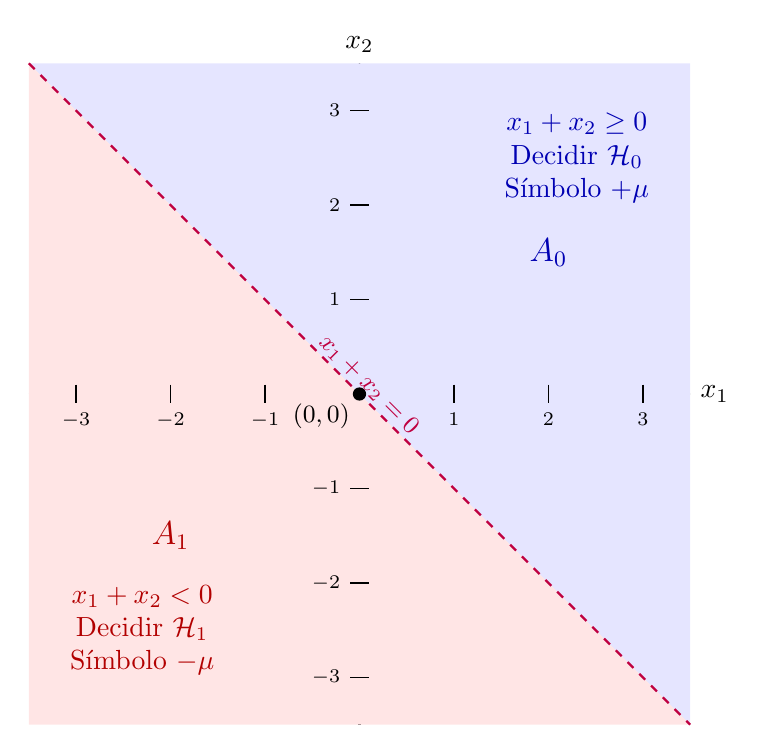
\begin{tikzpicture}[scale=1.2]
      % Ejes
      \draw[->, thick] (-3.5,0) -- (3.5,0) node[right] {$x_1$};
      \draw[->, thick] (0,-3.5) -- (0,3.5) node[above] {$x_2$};
      
      % Regiones de decisión (sombreadas)
      % Región azul A_0: donde x_1 + x_2 >= 0 (arriba/derecha de la diagonal)
      \fill[blue!10] (-3.5,3.5) -- (3.5,3.5) -- (3.5,-3.5) -- (-3.5,3.5) -- cycle;
      % Región roja A_1: donde x_1 + x_2 < 0 (abajo/izquierda de la diagonal)
      \fill[red!10] (-3.5,-3.5) -- (3.5,-3.5) -- (-3.5,3.5) -- cycle;
      
      % Frontera de decisión
      \draw[thick, purple, dashed] (-3.5,3.5) -- (3.5,-3.5);
      
      % Etiquetas de regiones
      \node[blue!70!black, font=\large\bfseries] at (2,1.5) {$A_0$};
      \node[red!70!black, font=\large\bfseries] at (-2,-1.5) {$A_1$};
      
      % Anotaciones
      \node[blue!70!black, align=center] at (2.3,2.5) {$x_1 + x_2 \geq 0$\\Decidir $\mathcal{H}_0$\\Símbolo $+\mu$};
      \node[red!70!black, align=center] at (-2.3,-2.5) {$x_1 + x_2 < 0$\\Decidir $\mathcal{H}_1$\\Símbolo $-\mu$};
      
      % Etiqueta de frontera
      \node[purple, font=\small, rotate=-45] at (0.1,0.1) {$x_1 + x_2 = 0$};
      
      % Punto origen
      \fill[black] (0,0) circle (2pt);
      \node[below left, font=\small] at (0,0) {$(0,0)$};
      
      % Marcas en los ejes
      \foreach \x in {-3,-2,-1,1,2,3}
      \draw (\x,0.1) -- (\x,-0.1) node[below, font=\scriptsize] {$\x$};
      \foreach \y in {-3,-2,-1,1,2,3}
      \draw (0.1,\y) -- (-0.1,\y) node[left, font=\scriptsize] {$\y$};
      
      \end{tikzpicture}
      \caption{Regiones de decisión en el plano $(x_1, x_2)$ para señalización antipodal con $n=2$ y $\eta=0$. La frontera de decisión $x_1 + x_2 = 0$ divide el plano en dos semiplanos: la región $A_0$ (azul) donde se decide el símbolo $+\mu$, y la región $A_1$ (roja) donde se decide el símbolo $-\mu$.}
      \label{fig:regiones_decision_antipodal}
      \end{figure}
      
      \subsection*{Resolución 2.3}
      
      Para resolver esta parte, necesitamos determinar el test óptimo para cada valor de $n$ tal que la probabilidad de falsa alarma sea $\alpha = 0.01$, y luego calcular la potencia del test (probabilidad de detección correcta) $\beta_\eta^*$. En la resolución 2.2, encontramos que el logaritmo del cociente de verosimilitud es:
      \begin{equation}
      \log(L(x_1^n)) = \frac{-2}{\sigma^2} \bar{\mu}^T \cdot x_1^n = \frac{-2\mu}{\sigma^2} \sum_{i=1}^n x_i
      \end{equation}
      
      Esto nos dice que la regla de decisión óptima solo depende de la suma $\sum_{i=1}^n x_i$, no de los valores individuales de cada $x_i$. 
      
      Para el caso particular de $n=2$ y $\eta=0$, obtuvimos la regla:
      \begin{equation}
      \text{Decidir } \mathcal{H}_1 \text{ si } x_1 + x_2 < 0
      \end{equation}
      
      Esto se puede generalizar para cualquier $n$ y cualquier umbral $\eta$. La regla de decisión de Neyman-Pearson es:
      \begin{equation}
      \log(L(x_1^n)) > \eta \quad \Leftrightarrow \quad \frac{-2\mu}{\sigma^2} \sum_{i=1}^n x_i > \eta
      \end{equation}
      
      Multiplicando ambos lados por $\frac{-\sigma^2}{2\mu}$ (y cambiando la dirección de la desigualdad porque multiplicamos por un número negativo):
      \begin{equation}
      \sum_{i=1}^n x_i < \frac{-\eta \sigma^2}{2\mu} \equiv \gamma
      \end{equation}
      
      donde hemos definido $\gamma = \frac{-\eta \sigma^2}{2\mu}$ como el umbral transformado. Por lo tanto, la regla de decisión óptima es:
      \begin{equation}
      \boxed{\text{Decidir } \mathcal{H}_1 \text{ si } \sum_{i=1}^n X_i < \gamma}
      \end{equation}
     
      
      La notación $X_1^n$ es una forma compacta de escribir la secuencia de observaciones $(X_1, X_2, \ldots, X_n)$. Es decir:
      \begin{equation}
      X_1^n \equiv (X_1, X_2, X_3, \ldots, X_n)
      \end{equation}
      
      Cada $X_i$ representa una medición individual. Por ejemplo, si $n=3$, entonces $X_1^3 = (X_1, X_2, X_3)$. Ademas podemos definir el estadístico $T(X_1^n)$ el cual es simplemente la \textbf{suma de todas las observaciones}:
      \begin{equation}
      T(X_1^n) = \sum_{i=1}^n X_i = X_1 + X_2 + X_3 + \cdots + X_n
      \end{equation}
      
      Este estadístico es suficiente porque resume toda la información relevante de las $n$ mediciones para tomar la decisión óptima. Bajo la hipótesis nula ($\theta = 0$, símbolo $+\mu$), cada observación es $X_i = \mu + N_i$, donde $N_i \sim \mathcal{N}(0, \sigma^2)$. Entonces:
      \begin{equation}
      T \left((X_1^n) | \theta = 0\right) = \sum_{i=1}^n X_i = \sum_{i=1}^n (\mu + N_i) = n\mu + \sum_{i=1}^n N_i
      \end{equation}
      
      Como la suma de variables normales independientes es también normal, tenemos:
      \begin{equation}
      T\left((X_1^n) | \theta = 0\right) \sim \mathcal{N}(n\mu, n\sigma^2)
      \end{equation}
      \begin{itemize}
      \item \textit{Media:} $n\mu$ (porque sumamos $n$ términos iguales a $\mu$, más ruidos que promedian a cero)
      
      \item \textit{Varianza:} $n\sigma^2$ (porque sumamos $n$ ruidos independientes, cada uno con varianza $\sigma^2$)
      \end{itemize}
      Análogamente, bajo la hipótesis alternativa ($\theta = 1$, símbolo $-\mu$), cada observación es $X_i = -\mu + N_i$:
      \begin{equation}
      T\left((X_1^n) | \theta = 1\right) = \sum_{i=1}^n (-\mu + N_i) = -n\mu + \sum_{i=1}^n N_i \sim \mathcal{N}(-n\mu, n\sigma^2)
      \end{equation}
      
      Para analizar con $\alpha = 0.01$, necesitamos encontrar el umbral $\gamma$ tal que:
      \begin{equation}
      \mathbb{P}_{H_0}(T(X_1^n) < \gamma) = \alpha = 0.01
      \end{equation}

      
      Sabemos que bajo $\mathcal{H}_0$, la suma $T(X_1^n) \sim \mathcal{N}(n\mu, n\sigma^2)$. El problema es que trabajar con distintas medias y varianzas es complicado. La \textbf{estandarización} es un truco matemático que convierte cualquier variable normal en una \textit{normal estándar} $\mathcal{N}(0,1)$ (media 0 y varianza 1), que está tabulada.
    
      Si $Y \sim \mathcal{N}(\mu_Y, \sigma_Y^2)$, entonces la variable estandarizada:
      \begin{equation}
      Z = \frac{Y - \mu_Y}{\sigma_Y} \sim \mathcal{N}(0,1)
      \end{equation}
      
      En nuestro caso, $Y = T(X_1^n)$ con media $\mu_Y = n\mu$ y desviación estándar $\sigma_Y = \sqrt{n\sigma^2} = \sigma\sqrt{n}$. Entonces:
      
      \begin{equation}
      Z = \frac{T(X_1^n) - n\mu}{\sigma\sqrt{n}} \sim \mathcal{N}(0,1)
      \end{equation}
      
      Aplicando esta transformación a la desigualdad $T(X_1^n) < \gamma$:
      \begin{align}
      \mathbb{P}_{H_0}(T(X_1^n) < \gamma) &= \mathbb{P}_{H_0}\left(\frac{T(X_1^n) - n\mu}{\sigma\sqrt{n}} < \frac{\gamma - n\mu}{\sigma\sqrt{n}}\right) \\
      &= \mathbb{P}\left(Z < \frac{\gamma - n\mu}{\sigma\sqrt{n}}\right) = \alpha
      \end{align}
      
      donde $Z \sim \mathcal{N}(0,1)$ es una normal estándar.

      Sabemos que $\mathbb{P}(Z < -z_\alpha) = \alpha$ donde $z_\alpha$ es el cuantil de la normal estándar. Para $\alpha = 0.01$, tenemos $z_{0.01} \approx 2.326$ (este valor se obtiene de tablas o software estadístico).
      
      Entonces:
      \begin{equation}
      \frac{\gamma - n\mu}{\sigma\sqrt{n}} = -z_\alpha \quad \Rightarrow \quad \gamma = n\mu - z_\alpha \sigma \sqrt{n}
      \end{equation}
      
      El umbral $\gamma$ está $z_\alpha = 2.326$ desviaciones estándar por debajo de la media bajo $\mathcal{H}_0$. Esto garantiza que la probabilidad de error tipo I (falsa alarma) sea exactamente $0.01$. La potencia $\beta_\eta^*$ es la probabilidad de decidir correctamente $\mathcal{H}_1$ cuando $\mathcal{H}_1$ es verdadera:
      \begin{equation}
      \beta_\eta^* = \mathbb{P}_{H_1}(T(X_1^n) < \gamma)
      \end{equation}
      
      Bajo $\mathcal{H}_1$, sabemos que $T(X_1^n) \sim \mathcal{N}(-n\mu, n\sigma^2)$. Estandarizamos nuevamente, pero ahora usando la media y varianza bajo $\mathcal{H}_1$:
      
      \begin{align}
      \beta_\eta^* &= \mathbb{P}_{H_1}(T(X_1^n) < \gamma) \\
      &= \mathbb{P}_{H_1}\left(\frac{T(X_1^n) - (-n\mu)}{\sigma\sqrt{n}} < \frac{\gamma - (-n\mu)}{\sigma\sqrt{n}}\right) \\
      &= \mathbb{P}_{H_1}\left(\frac{T(X_1^n) + n\mu}{\sigma\sqrt{n}} < \frac{\gamma + n\mu}{\sigma\sqrt{n}}\right) \\
      &= \mathbb{P}\left(Z < \frac{\gamma + n\mu}{\sigma\sqrt{n}}\right)
      \end{align}
      
      donde $Z \sim \mathcal{N}(0,1)$. Ahora sustituimos $\gamma = n\mu - z_\alpha \sigma\sqrt{n}$:
      
      \begin{align}
      \beta_\eta^* &= \mathbb{P}\left(Z < \frac{(n\mu - z_\alpha \sigma\sqrt{n}) + n\mu}{\sigma\sqrt{n}}\right) \\
      &= \mathbb{P}\left(Z < \frac{2n\mu - z_\alpha \sigma\sqrt{n}}{\sigma\sqrt{n}}\right) \\
      &= \mathbb{P}\left(Z < \frac{2n\mu}{\sigma\sqrt{n}} - z_\alpha\right) \\
      &= \mathbb{P}\left(Z < \frac{2\mu\sqrt{n}}{\sigma} - z_\alpha\right)
      \end{align}
      
      donde $Z \sim \mathcal{N}(0,1)$ es una variable aleatoria normal estándar. Esta probabilidad se puede calcular usando tablas de la distribución normal o software estadístico.


      
      Con $\mu = 1$, $\sigma^2 = 10$ (por lo tanto $\sigma = \sqrt{10} \approx 3.162$), y $z_{0.01} \approx 2.326$:
      
      \begin{align}
      n = 1: \quad & \beta^* = \mathbb{P}\left(Z < \frac{2 \cdot 1 \cdot 1}{3.162} - 2.326\right) = \mathbb{P}(Z < -1.694) \approx 0.045 \\
      n = 10: \quad & \beta^* = \mathbb{P}\left(Z < \frac{2 \cdot 1 \cdot \sqrt{10}}{3.162} - 2.326\right) = \mathbb{P}(Z < -0.326) \approx 0.372 \\
      n = 100: \quad & \beta^* = \mathbb{P}\left(Z < \frac{2 \cdot 1 \cdot 10}{3.162} - 2.326\right) = \mathbb{P}(Z < 3.999) \approx 1.000 \\
      n = 1000: \quad & \beta^* = \mathbb{P}\left(Z < \frac{2 \cdot 1 \cdot \sqrt{1000}}{3.162} - 2.326\right) = \mathbb{P}(Z < 17.674) \approx 1.000
      \end{align}
      
  Algunos aspectos importantes a destacar:
      
      \begin{itemize}
      \item \textbf{Efecto del número de mediciones:} La potencia del test $\beta^*$ aumenta significativamente con el número de mediciones $n$. Con una sola medición ($n=1$), la potencia es apenas $4.5\%$. Con $n=10$ mediciones, la potencia aumenta a $37.2\%$. Con $n=100$ mediciones, la potencia es prácticamente $100\%$.
      
      \item \textbf{Ventaja de la señalización antipodal:} Comparado con señalización ON-OFF (donde un símbolo es cero), la señalización antipodal aprovecha mejor la energía disponible, ya que ambos símbolos están a distancia $\mu$ del origen. La distancia efectiva entre símbolos es $2\mu$, lo que duplica la capacidad de discriminación.
      
      \item \textbf{Relación con $\sqrt{n}$:} La potencia mejora con $\sqrt{n}$ debido a que la varianza del promedio decrece como $1/n$, mientras que la diferencia entre medias escala con $n$.
      

      \end{itemize}
      
      \subsection*{Resolución 2.4}
      
      Para generar la curva ROC completa, debemos analizar cómo varía la potencia del test $\beta$ (probabilidad de detección) en función del tamaño del test $\alpha$ (probabilidad de falsa alarma) para diferentes valores de $n$.
      
      
      La curva ROC se construye graficando $\beta(\alpha)$ versus $\alpha$ para $\alpha \in [0,1]$. Para un tamaño de test $\alpha$ dado, el umbral es:
      \begin{equation}
      \gamma = n\mu - z_\alpha \sigma \sqrt{n}
      \end{equation}
      
      donde $z_\alpha$ es el cuantil de orden $1-\alpha$ de la distribución normal estándar tal que $\mathbb{P}(Z \leq z_\alpha) = 1-\alpha$ (equivalentemente, $\mathbb{P}(Z < -z_\alpha) = \alpha$). La potencia del test correspondiente es:
      \begin{equation}
      \beta(\alpha) = \mathbb{P}_{H_1}(T(X_1^n) < \gamma) = \mathbb{P}\left(Z < \frac{2\mu\sqrt{n}}{\sigma} - z_\alpha\right)
      \end{equation}
      
      De esta forma, obtenemos la curva ROC que relaciona $\beta$ y $\alpha$:
      \begin{equation}
      \beta(\alpha) = \mathbb{P}\left(Z < \frac{2\mu\sqrt{n}}{\sigma} - z_{1-\alpha}\right)
      \end{equation}
      
      donde $z_{1-\alpha}$ es el cuantil de orden $1-\alpha$ de la distribución normal estándar $Z \sim \mathcal{N}(0,1)$ (es decir, $\mathbb{P}(Z \leq z_{1-\alpha}) = 1-\alpha$).
      
      Equivalentemente:
      \begin{equation}
      \beta(\alpha) = \mathbb{P}\left(Z < z_{\alpha} + \frac{2\mu\sqrt{n}}{\sigma}\right)
      \end{equation}
      
      donde $z_{\alpha}$ es el cuantil de orden $\alpha$ de la distribución normal estándar.
      
      
      La curva ROC tiene las siguientes propiedades importantes:
      
      \begin{itemize}
      \item \textbf{Punto (0,0):} Corresponde a un test que nunca rechaza $\mathcal{H}_0$ (decisión trivial: siempre aceptar $\mathcal{H}_0$). Se tiene $\alpha = 0$ y $\beta = 0$.
      
      \item \textbf{Punto (1,1):} Corresponde a un test que siempre rechaza $\mathcal{H}_0$ (decisión trivial: siempre decidir $\mathcal{H}_1$). Se tiene $\alpha = 1$ y $\beta = 1$.
      
      \item \textbf{Diagonal $\beta = \alpha$:} Representa un test aleatorio sin información (equivalente a lanzar una moneda). Un buen test debe estar por encima de esta diagonal.
      
      \item \textbf{Punto de operación anterior ($\alpha = 0.01$):} Este es el punto específico analizado en la parte 2.3, donde fijamos $\alpha = 0.01$ y calculamos los valores de $\beta$ correspondientes.
      \end{itemize}
      
      A continuación, se presentan las curvas ROC para los diferentes valores de $n$ (1, 10, 100, 1000) con $\mu = 1$ y $\sigma^2 = 10$. Cada curva se genera variando $\alpha$ desde 0 hasta 1 y calculando el correspondiente $\beta(\alpha)$.
      
      \begin{enumerate}
      \item \textbf{$n = 1$:}
      
      Con una sola medición en señalización antipodal, la curva ROC muestra una capacidad de discriminación limitada pero mejor que el caso unipolar. Para $\alpha = 0.01$, obtuvimos $\beta \approx 0.045$, lo que significa que la probabilidad de detectar correctamente el símbolo $-\mu$ es del 4.5\%.
      
      El área bajo la curva (AUC) para este caso es aproximadamente 0.58, indicando rendimiento modesto pero mejor que el azar.
      
      \item \textbf{$n = 10$:}
      
      Con 10 mediciones, la curva ROC se aleja notablemente de la diagonal. Para $\alpha = 0.01$, tenemos $\beta \approx 0.372$, mejorando significativamente la capacidad de detección. El AUC aumenta considerablemente a aproximadamente 0.79.
      
      \item \textbf{$n = 100$:}
      
      Con 100 mediciones, la curva ROC se acerca mucho a la esquina superior izquierda (punto ideal (0,1)). Para $\alpha = 0.01$, tenemos $\beta \approx 1.000$, lo que significa que podemos detectar la señal con probabilidad casi perfecta manteniendo una tasa de falsa alarma muy baja.
      
      El AUC es mayor a 0.99, indicando un excelente rendimiento.
      
      \item \textbf{$n = 1000$:}
      
      Con 1000 mediciones, la curva ROC es prácticamente una línea que va de (0,0) a (0,1) y luego a (1,1), siguiendo el eje vertical y luego el horizontal. Para $\alpha = 0.01$, tenemos $\beta \approx 1.0$, lo que significa detección perfecta.
      
      El AUC es prácticamente 1, indicando rendimiento perfecto.
      \end{enumerate}
    
      
      \begin{figure}[H]
      \centering
      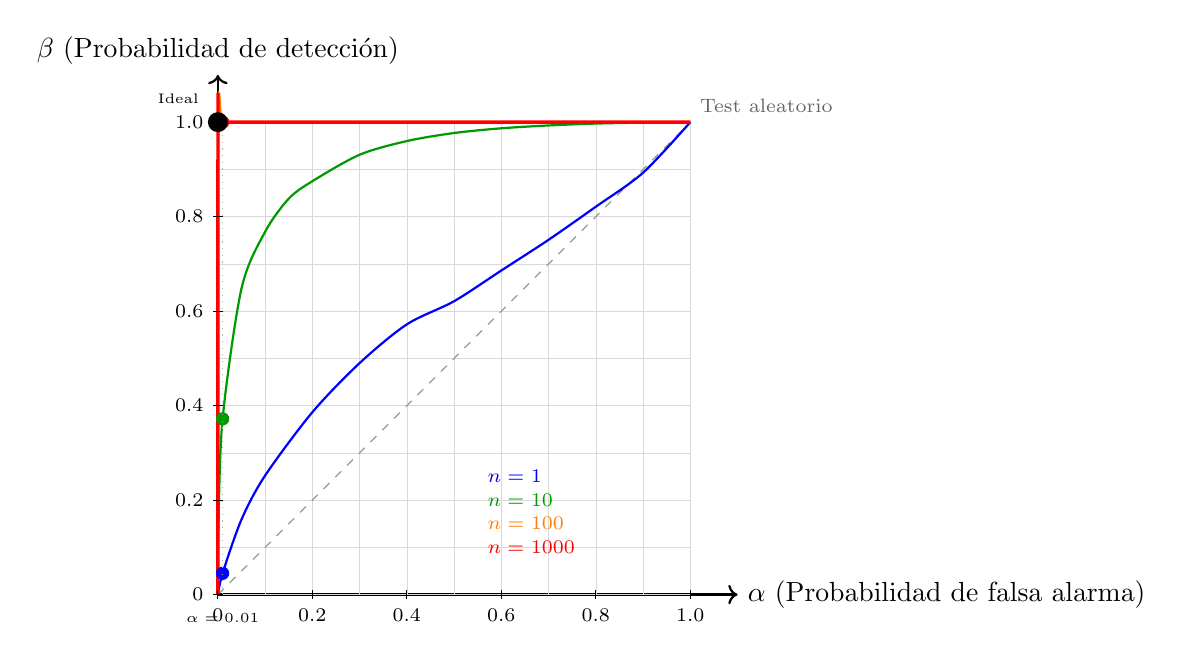
\begin{tikzpicture}[scale=6]
      % Ejes
      \draw[->, thick] (0,0) -- (1.1,0) node[right] {$\alpha$ (Probabilidad de falsa alarma)};
      \draw[->, thick] (0,0) -- (0,1.1) node[above] {$\beta$ (Probabilidad de detección)};
      
      % Grilla
      \draw[gray!30, very thin] (0,0) grid[step=0.1] (1,1);
      
      % Diagonal (test aleatorio sin información)
      \draw[black!40, dashed, thin] (0,0) -- (1,1) node[above right, font=\scriptsize, black!60] {Test aleatorio};
      
      % Curvas ROC (aproximadas usando curvas suaves)
      % n=1 (SNR=0.632) - curva cercana a la diagonal
      \draw[blue, thick, smooth] 
        plot coordinates {
          (0,0) (0.01,0.045) (0.05,0.159) (0.1,0.252) (0.2,0.386) 
          (0.3,0.490) (0.4,0.572) (0.5,0.621) (0.6,0.686) (0.7,0.751) 
          (0.8,0.821) (0.9,0.893) (1,1)
        };
      
      % n=10 (SNR=2.0) - curva intermedia
      \draw[green!60!black, thick, smooth] 
        plot coordinates {
          (0,0) (0.001,0.135) (0.01,0.372) (0.05,0.648) (0.1,0.768) 
          (0.15,0.838) (0.2,0.875) (0.3,0.931) (0.4,0.960) (0.5,0.977) 
          (0.6,0.987) (0.7,0.993) (0.8,0.997) (0.9,0.999) (1,1)
        };
      
      % n=100 (SNR=6.325) - curva muy cercana a la ideal
      \draw[orange, thick, smooth] 
        plot coordinates {
          (0,0) (0.001,0.999) (0.01,1.0) (0.05,1.0) (0.1,1.0) 
          (0.2,1.0) (0.5,1.0) (1,1)
        };
      
      % n=1000 (SNR=20.0) - prácticamente ideal
      \draw[red, very thick, smooth] 
        plot coordinates {
          (0,0) (0.0001,1.0) (0.001,1.0) (0.01,1.0) (0.1,1.0) (1,1)
        };
      
      % Punto de operación α=0.01 marcado
      \fill[blue] (0.01,0.045) circle (0.4pt);
      \fill[green!60!black] (0.01,0.372) circle (0.4pt);
      \fill[orange] (0.01,1.0) circle (0.4pt);
      \fill[red] (0.01,1.0) circle (0.4pt);
      
      % Línea vertical en α=0.01
      \draw[black!30, dotted] (0.01,0) -- (0.01,1);
      \node[below, font=\tiny] at (0.01,-0.02) {$\alpha=0.01$};
      
      % Leyenda
      \node[blue, font=\scriptsize, anchor=west] at (0.55, 0.25) {$n=1$};
      \node[green!60!black, font=\scriptsize, anchor=west] at (0.55, 0.20) {$n=10$};
      \node[orange, font=\scriptsize, anchor=west] at (0.55, 0.15) {$n=100$};
      \node[red, font=\scriptsize, anchor=west] at (0.55, 0.10) {$n=1000$};
      
      % Marcas en los ejes
      \foreach \x in {0, 0.2, 0.4, 0.6, 0.8, 1.0}
      \draw (\x,0.01) -- (\x,-0.01) node[below, font=\scriptsize] {\x};
      \foreach \y in {0, 0.2, 0.4, 0.6, 0.8, 1.0}
      \draw (0.01,\y) -- (-0.01,\y) node[left, font=\scriptsize] {\y};
      
      % Punto ideal (0,1)
      \fill[black] (0,1) circle (0.6pt);
      \node[left, font=\tiny] at (-0.02,1.05) {Ideal};
      
      \end{tikzpicture}
      \caption{Curvas ROC para detección de señalización antipodal con diferentes números de mediciones $n$. A medida que $n$ aumenta, las curvas se desplazan hacia el punto ideal (0,1), indicando mejor discriminación entre las hipótesis. La línea punteada vertical marca el punto de operación analizado en la parte 2.3 con $\alpha=0.01$.}
      \label{fig:curvas_roc_antipodal}
      \end{figure}
    \end{solution}
    %----------------------
    
\end{questions}
\end{document}